\label{chap:discussion}

 

\section{Lengths of Tracks}
\label{section:lengthoftracks}


\begin{figure}
		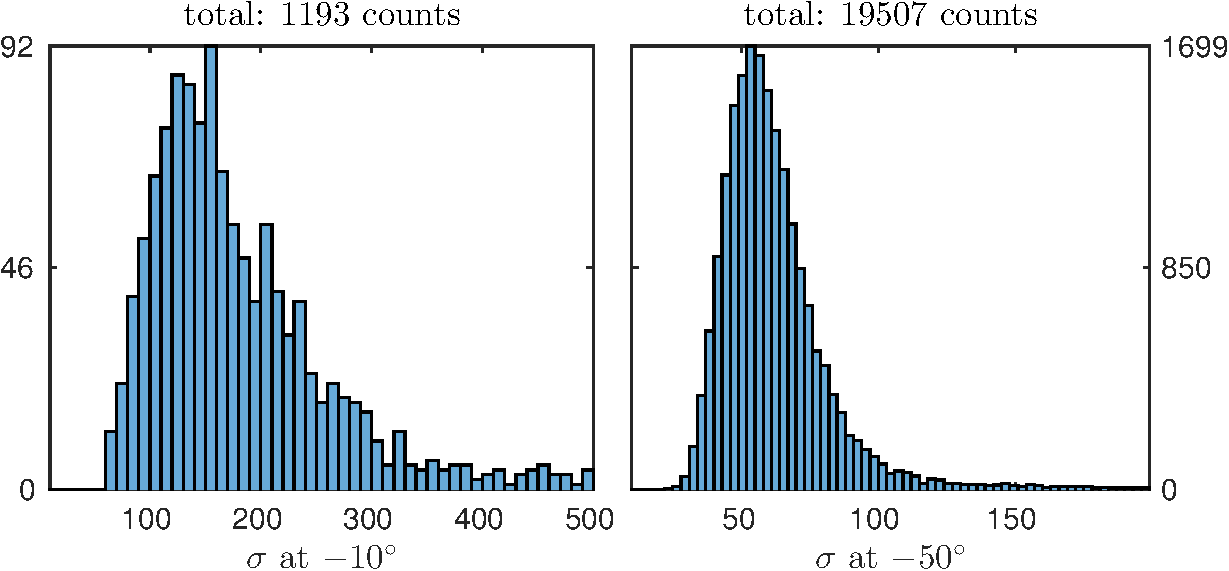
\includegraphics[]{hist-sigmaAt-both-aviI}
		\caption{\aviI \capS. Histograms of $\scale$ at a low and a high latitude.}
	\label{fig:hist-sigmaAt-both-aviI}
\end{figure}

\newthought{The}~most apparent difference between the results of the \href{box:MI}{two detection-methods} is the abundance of long-lived eddies resulting from the \MI-method.
This discrepancy must logically be caused by the two different contour-shape testing-procedures (see \cref{box:MII,filter:shape}), since it is here where the main difference between the two methods' algorithms lies.

\newthought{The } \MI-method is the more lenient one, as all it checks for is whether the contour is of sufficiently compact form. The only shapes that are dismissed are long, thin elongated structures. This means that \eg an eddy track can more easily \footnote{as long as the similarity-criterion is not violated.} survive situations in which two eddies merge into one or those in which one is split into two or situations in which mean current gradients distort the vortex (see \cref{fig:parAnalyCH}). There could also be the situation in which an old, weak eddy fades, yet another one emerges in sufficient proximity. These two events would not even have to coincide at the exact same time, as long as some short-lived coherent structure, of which there is an abundance \footnote{see \cref{fig:allEddies-aviIaviIIpop7II}} at any given time-step throughout the world ocean, acted as a \textit{bridge} to fill the gap.
%\TODO{chelton is really just tracking closed contours encompassing some area of uniform ssh sign... no shape requirement whatsoever..}



\begin{figure*}
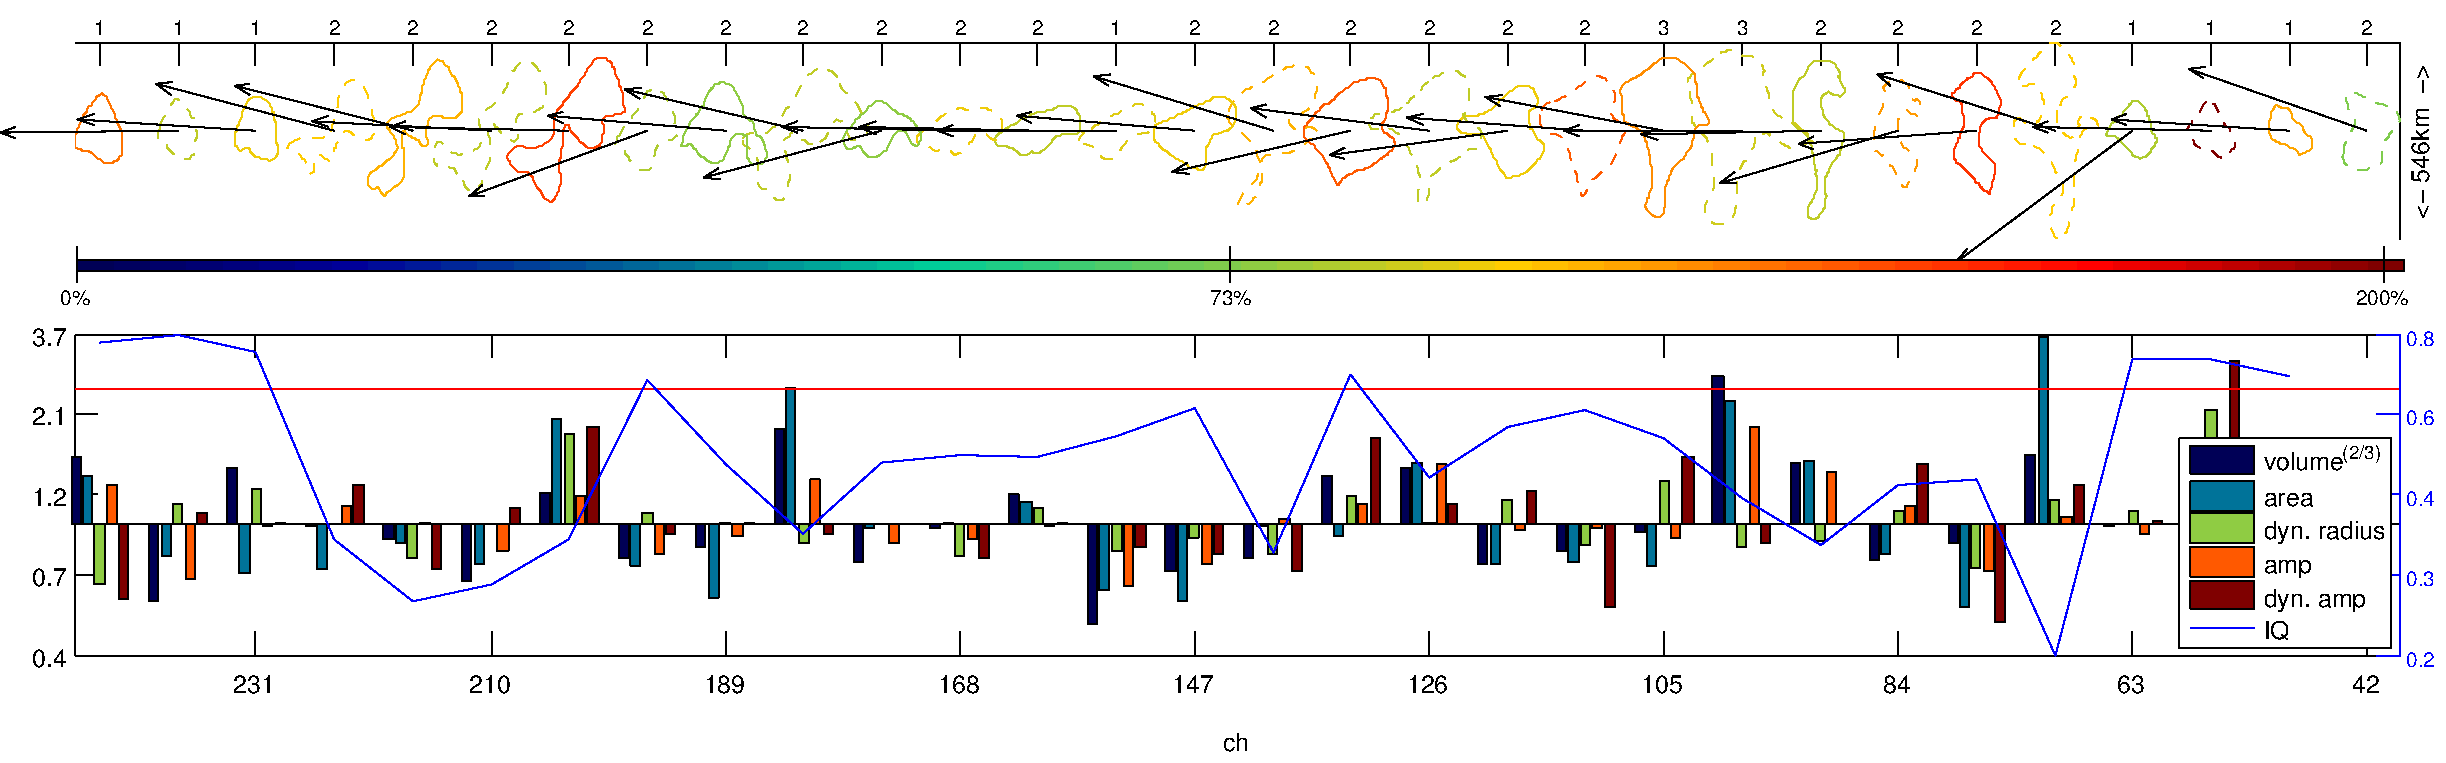
\includegraphics[]{parAnalyCH}
\caption{The \MI-method. Top: Consecutive contours of one track. Colors indicate percentage of change of contour's area with respect to the prior time-step. Topmost horizontal axis shows the (rounded) factor of $\scale$ with respect to the local first baroclinic $\Lr$. Vectors' lengths are proportional to the distance traveled with respect to the next time-step. Bottom: Blue graph shows the current $\IQ$. Bars show the factors of change of respective parameters with respect to the prior time-step. X-axis are days since birth.}
\label{fig:parAnalyCH}
\end{figure*}

\newthought{The } \MII-method is conceptually different in that it is based on the assumption that a distinct coherent vortex need \textit{per definition} to be more or less circular. It will therefor be more likely to regard \eg the situation in which one eddy merges with another as a situation of 3 eddies in total; \textbf{two} that have just died to create \textbf{one} new one.
The focus here is more on the propagation of distinct circular geostrophic vortices whereas the focus in the \MI-method is more general on coherent local depressions respective elevations in \SSH (see \cref{fig:parAnalyIQ6}).
It should be interesting to look at to which degree tracers found within tracked eddies remain within the eddy over time (postponed for now). This could further clarify the hypothesis that the \MI-method might be better at tracking water-mass advecting entities, with less jumps between bodies of water within one track. \Eg looking at temperature/salt at the eddy's core as a function of time. The downside of the $\IQ$-method is that the identity checks between time-steps fail more easily in the case of merging/splitting situations, thus cutting tracks short. \Ie in the case of one large eddy absorbing another, it does not \textit{die}, but its contour becomes temporarily disfigured and it might thus fail the id check.
It comes again down to a question of definition \ie if one large eddy splits into two small ones are we talking about three, or two unique eddies in total?

\begin{figure*}
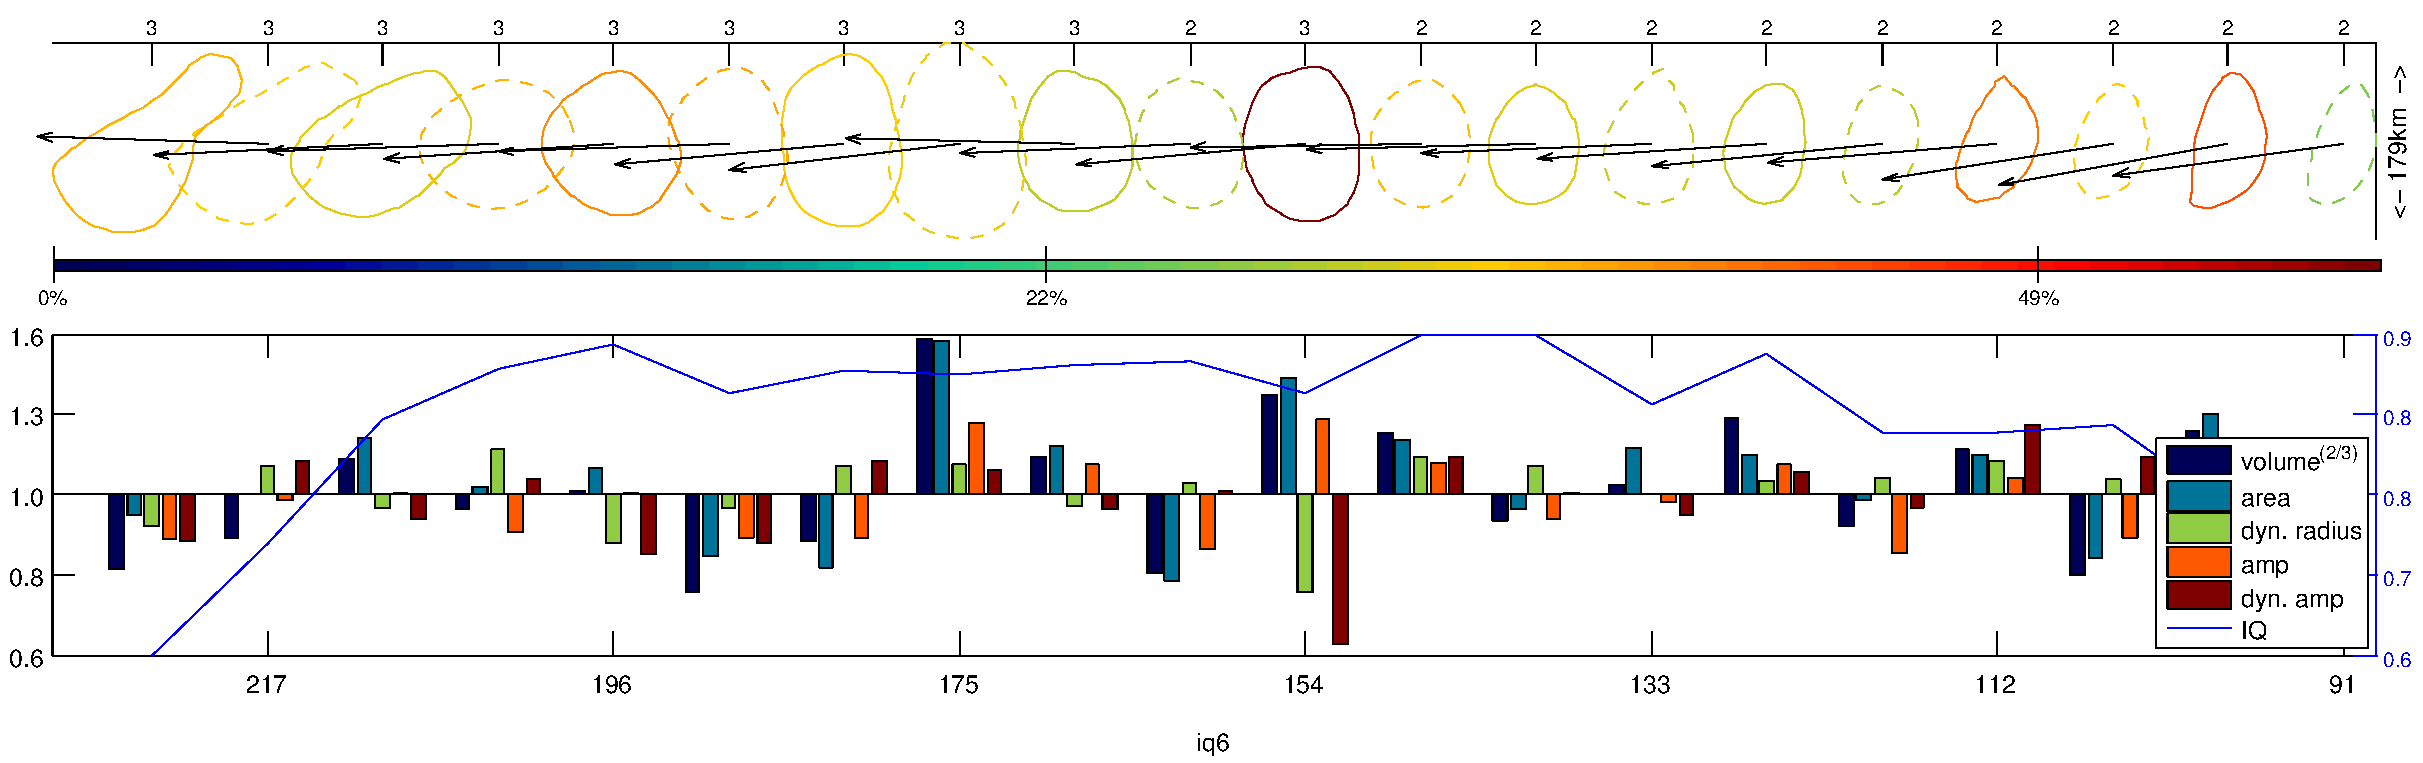
\includegraphics[]{parAnalyIQ6}
\caption{The \MII-method ($\IQ$-threshold at $0.6$). (see \cref{fig:parAnalyCH})}
\label{fig:parAnalyIQ6}
\end{figure*}




% %%%%%%%%%%%%%%%%%%%%%%%%%%%%%%%%%%%%%%%%%%%%%%%%%%%%%%%%%%%%%%%%%%%%%%%%%%%%%%%%%% %%%%%%%%%%%%%%%%%%%%%%%%%%%%%%%%%%%%%%%%%%%%%%%%%%%%%%%%%%%%%%%%%%%%%%%%%%%%%%%%%% %%%%%%%%%%%%%%%%%%%%%%%%%%%%%%%%%%%%%%%%%%%%%%%%%%%%%%%%%%%%%%%%%%%%%%%%%%%%%%%%%% %%%%%%%%%%%%%%%%%%%%%%%%%%%%%%%%%%%%%%%%%%%%%%%%%%%%%%%%%%%%%%%%%%%%%%%%%%%%%%%%%

\section{Scales and the Effect of Down-Sampling}
\label{sec:downsampled}

% %%%%%%%%%%%%%%%%%%%%%%%%%%%%%%%%%%%%%%%%%%%%%%%%%%%%%%%%%%%%%%%%%%%%%%%%%%%%%%%%%

\newthought{Interestingly }, even in the \aviI results, the horizontal eddy scale $\scale$ differs from that presented by \citet{Chelton2011}. For latitudes $\gtrsim\abs{\deg{25}}$ the zonal mean here is smaller than theirs while for low latitudes it is higher (see \cref{fig:ScheltsAll,fig:sigmaSatDiffsINTRSCT}). The reason for this discrepancy is suspected to stem from the special method by which $\scale$ is determined by our algorithm.
As outlined in \cref{filter:dynscale}, here $\scale$ is half the mean of zonal and meridional distances between the first two local extrema of the first derivative of interpolated 4th-order Fourier fits to the \SSH~data around the eddy's \CoV. \Citeauthor{Chelton2011} calculate the respective scale via \textit{a direct estimate based on the contour of \SSH within the eddy interior around which the average geostrophic speed is maximum}. \Ie they derive $\scale$ directly via the area described by the contour of maximum $\abs{\tvec{\grad} \vec{u}}$ and not via any Fourier-type fit.
 %Depending on implementation-details of the contour function they used,    
\begin{marginfigure}
	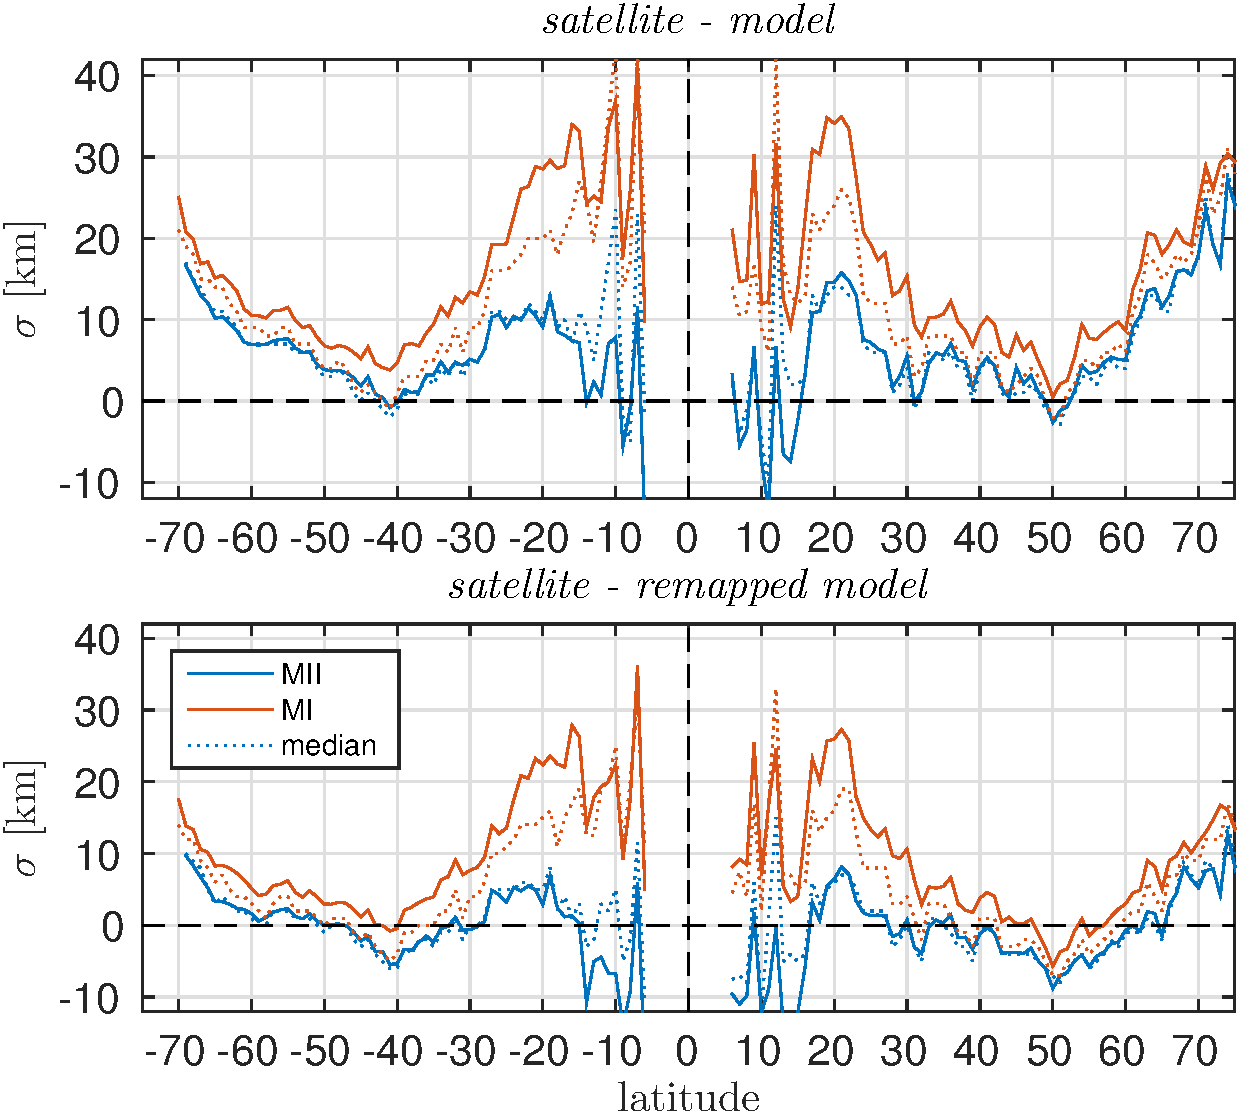
\includegraphics[]{sigmaSatDiffsINTRSCT}
	\caption{Differences in zonal mean $\scale$ between \AVI/\POP~and \AVI/down-sampled \POP. Means/Medians are built zonally over only those $\deg{1}\times\deg{1}$-bins that feature data in both sets \ie the intersection of $lat+1\i \; lon$ of both sets. }
	\label{fig:sigmaSatDiffsINTRSCT}
\end{marginfigure}

\newthought{The } motivation to use fits instead of the \SSH~directly was on the one hand to avoid noise complicating correct determinations of the 2nd differential zero-crossings and on the other hand to tackle the problem of coarse resolution, especially so for high latitudes where $\scale$ seems to become as small as only twice the distance between data points. At this resolution the \textit{Gaussian RMS width} of an eddy would amount to only 5 data points. Since $\scale$ is generally smaller in the higher-resolution \POP-data analyses, we hypothesize that the scales by \citeauthor{Chelton2011} are biased high for high latitudes. Question remains to what degree this bias is inherent to the \AVI~product \ie as a smearing effect from the interpolation of multiple coarse satellite data. Or whether it is attributable entirely to the particular method by which the diameter/area of the zero-vorticity contour is estimated.


% %%%%%%%%%%%%%%%%%%%%%%%%%%%%%%%%%%%%%%%%%%%%%%%%%%%%%%%%%%%%%%%%%%%%%%%%%%%%%%%%%
\begin{marginfigure}
	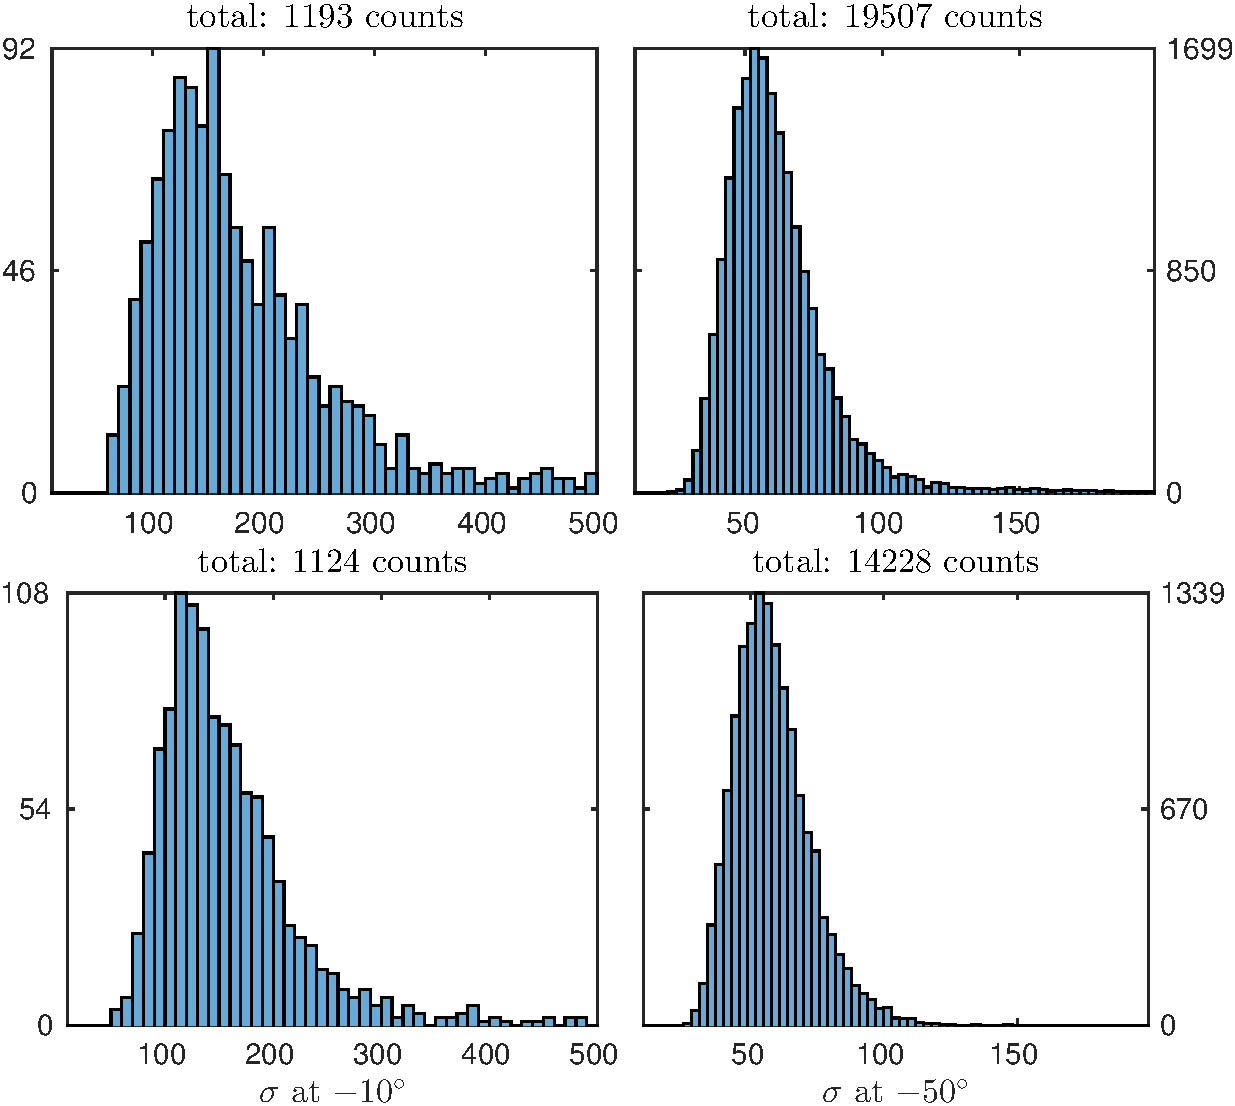
\includegraphics[]{hist-sigmaAt-both-aviIaviII}
	\caption{Eddy count at one point in time for one fully zonal $\deg{1}$-bin. Top: \aviI. Bottom: \aviII. The tropical spectrum is broad yet with strong positive skewness \ie oriented towards smaller scales. In high latitudes the standard deviation is smaller. The \MI method yields more large eddies.}
	\label{fig:hist-sigmaAt-both-aviIaviII}
\end{marginfigure}
% %%%%%%%%%%%%%%%%%%%%%%%%%%%%%%%%%%%%%%%%%%%%%%%%%%%%%%%%%%%%%%%%%%%%%%%%%%%%%%%%%

\newthought{With regard } to the lower latitudes two important aspects need to be considered:
\begin{enumerate}
	\item
	The analyses yield generally low eddy activity in the tropics. Hence the results are less robust in this region \textit{a priori}.
	\item
	The standard deviation in $\scale$ is particularly broad in the tropics (see \cref{fig:hist-sigmaAt-both-aviIaviII}). As a matter of fact it appears as though there might be two different types of eddies. One type analogous to all high-latitude eddies and a new one of much larger scale. Because these larger eddies have generally low $\IQ$-values they are filtered from the \MII~analyses, resulting in smaller tropical $\scale$. Their more chaotic shape might, due to the different methods to determine $\scale$, also have to do with why mean tropical $\scale$ is larger here than in \citet{Chelton2011}.
\end{enumerate}

 %%%%%%%%%%%%%%%%%%%%%%%%%%%%%%%%%%%%%%%%%%%%%%%%%%%%%%%%%%%%%%%%%%%%%%%%%%%%%%%%%%
%\begin{wrapfigure}{r}{.6\textwidth}
%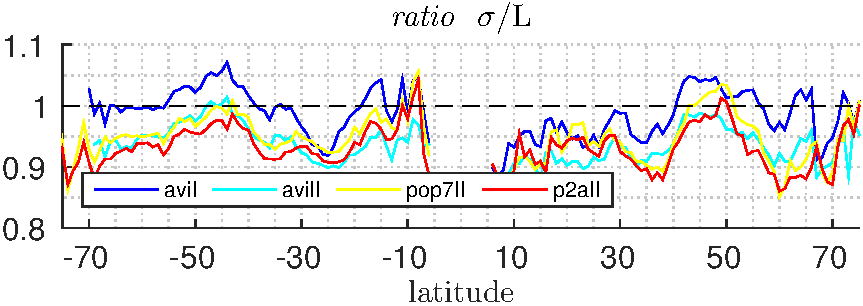
\includegraphics[width=0.6\textwidth]{S-scaleRatios-aviI}
%\caption{ Ratios of $\scale$ to $\mathrm{L}$  (see \cref{filter:chstuff}). In the ideal case of a perfect Gaussian profile, $\scale$ and $\mathrm{L}$ would be equivalent. \TODO{take out? Dont make no sense}}
%\label{fig:S-scaleRatios-aviI}
%\end{wrapfigure}
 %%%%%%%%%%%%%%%%%%%%%%%%%%%%%%%%%%%%%%%%%%%%%%%%%%%%%%%%%%%%%%%%%%%%%%%%%%%%%%%%%%

% %%%%%%%%%%%%%%%%%%%%%%%%%%%%%%%%%%%%%%%%%%%%%%%%%%%%%%%%%%%%%%%%%%%%%%%%%%%%%%%%%
\begin{marginfigure}[6.5cm]
	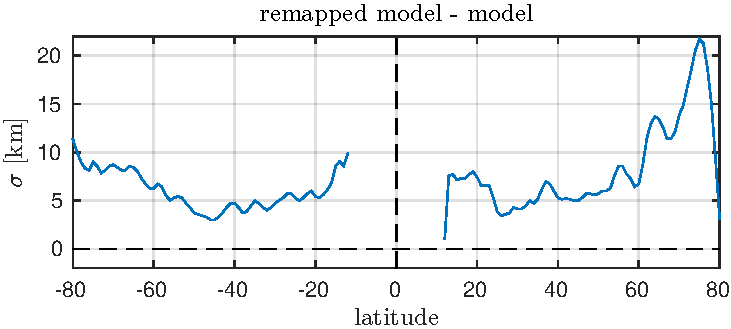
\includegraphics[]{sigmaP2aMinusMod}
	\caption{Difference in \Scale between \pToaII and \popSevenII.}
	\label{fig:sigmaP2aMinusMod}
\end{marginfigure}
% %%%%%%%%%%%%%%%%%%%%%%%%%%%%%%%%%%%%%%%%%%%%%%%%%%%%%%%%%%%%%%%%%%%%%%%%%%%%%%%%%
\newthought{The } \popSevenII analysis yields somewhat similar $\scale$ for low latitudes \footnote{Note that due to the lack of tropical eddies the estimates of $\scale$ are rather uncertain for the \POP~analyses.}, yet significantly smaller values for high latitudes. The question here therefor is whether this discrepancy is a result of the lower resolution of the satellite data \ie that eddies are too small to be resolved by the \AVI~product in high latitudes or whether it is attributable to the model data as in a systematic bias due to incomplete/poorly parameterized model physics. This question was the primary motivation for the \pToaII-run. The idea here was to down-size the \POP~data to the geometry of the \AVI~grid in order to test whether this would raise $\scale$ to that from the satellite results. \Cref{fig:sigmaSatDiffsINTRSCT} shows that the down-sampling did indeed decrease the discrepancy in $\scale$ to respective \AVI~analysis, as long as those regions that are unique to either data set are excluded. Between $\pm \deg{25}$ and $\pm \deg{65}$ the difference is no larger than $\pm \km{5}$. This came as a surprise because since $\scale$ stems from Fourier fits of SSH, we expected the original frequencies to be, at least to some extent, conserved in the down-sampled data (see also \cref{fig:sigmaP2aMinusMod}).

%% %%%%%%%%%%%%%%%%%%%%%%%%%%%%%%%%%%%%%%%%%%%%%%%%%%%%%%%%%%%%%%%%%%%%%%%%%%%%%%%%%
%\begin{marginfigure}
%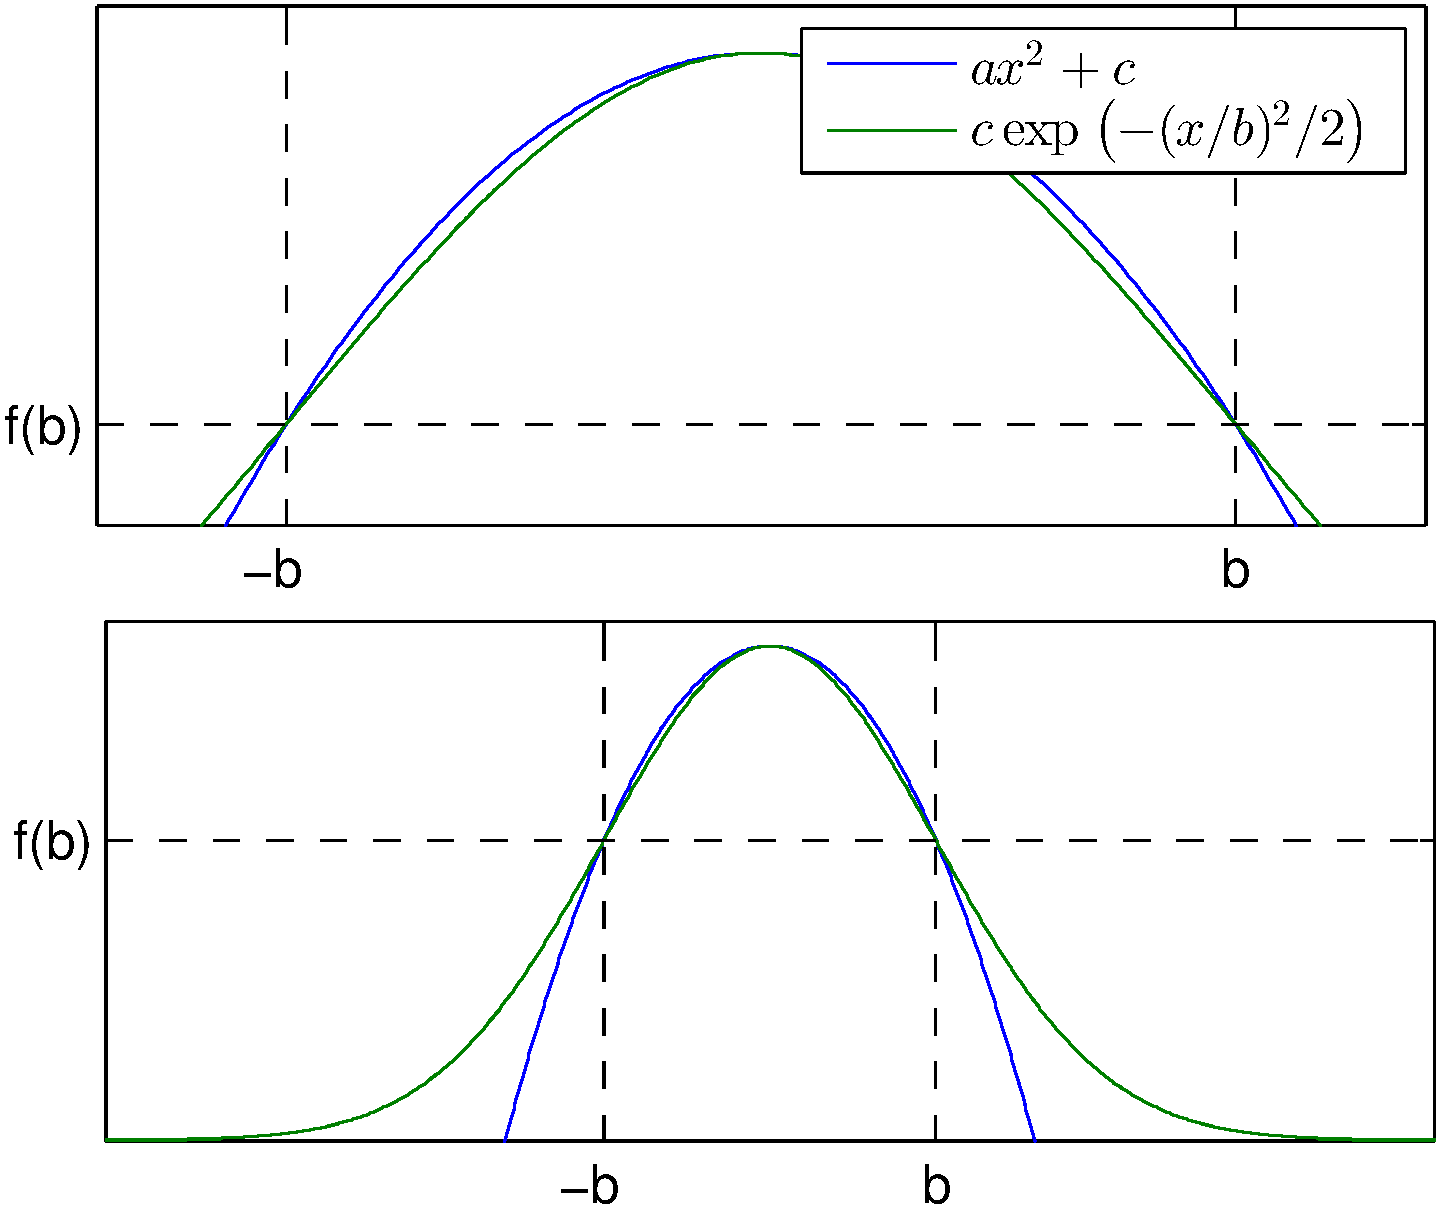
\includegraphics[]{gaussVSquadSmaller}
%\caption{The upper part of a Gaussian profile can appear similar to a quadratic one. \TODO{ref to here}}
%\label{fig:gaussVSquadSmaller}
%\end{marginfigure}
% %%%%%%%%%%%%%%%%%%%%%%%%%%%%%%%%%%%%%%%%%%%%%%%%%%%%%%%%%%%%%%%%%%%%%%%%%%%%%%%%%





%\section{Profiles}

 %\TODO{chelton The fact that $L_s$ is consistently so much larger than L is a clear indication of inadequacy of a
%Gaussian approximation for the eddy structures, in which case $L_s$ and $L$ would be equal as noted above. It is shown in Section 5 that the most frequently occurring structure of the tracked eddies consists approximately of an
%axisymmetric quadratic profile of \SSH within most of the radius Ls, thus resulting in Ls significantly larger than the scale L that would be obtained if the eddies had Gaussian shape.
%wrong! eddies not detect at base, hence only tip being looked at $\rightarrow$ seemingly quqdratic profile..
%}
%\newthought{The}~\MI detection method a priori assumes that an eddy is more or less detected at its asymptotic \textit{floor} \ie in the case of an \AC at the \textit{foot of the mountain}.
 %The idea of the $\IQ$-based method on the other hand is to assume that the situation of a single well-defined eddy sitting on an otherwise smooth, flat sea surface, which would be necessary for the contour algorithm to find a closed contour describing the outermost perimeter of said single vortex, is unrealistic. Instead the approach is to look for distinct, sufficiently circular \textit{caps} of SSH-hills/valleys that consistently \textit{wade} through all other weaker geostrophic noise surrounding it.

%\TODO{ why gaussian or quad? Read \citet{Zhang2013,beckers2001dynamics}}
%\TODO{explain
 %%\cref{fig:S-scaleRatios-aviI,fig:gaussVSquad}
 	%}


% %%%%%%%%%%%%%%%%%%%%%%%%%%%%%%%%%%%%%%%%%%%%%%%%%%%%%%%%%%%%%%%%%%%%%%%%%%%%%%%%%
\section{Drift Speeds}

\newthought{Zonal}~mean drift speeds of all \AVI~results agree well with those presented by \citet{Chelton2011} (see \cref{fig:ScheltsAll}), suggesting that the tracking procedures are relatively robust for both the \MI~and \MII~methods.

%%%%%%%%%%%%%%%%%%%%%%%%%%%%%%%%%%%%%%%%%%%%%%%%%%%%%%%%%%%%%%%%%%%%%%%%%%%%%%%%%
\begin{marginfigure}
	\label{fig:UsubSampledAviIAviIIPop7II}
	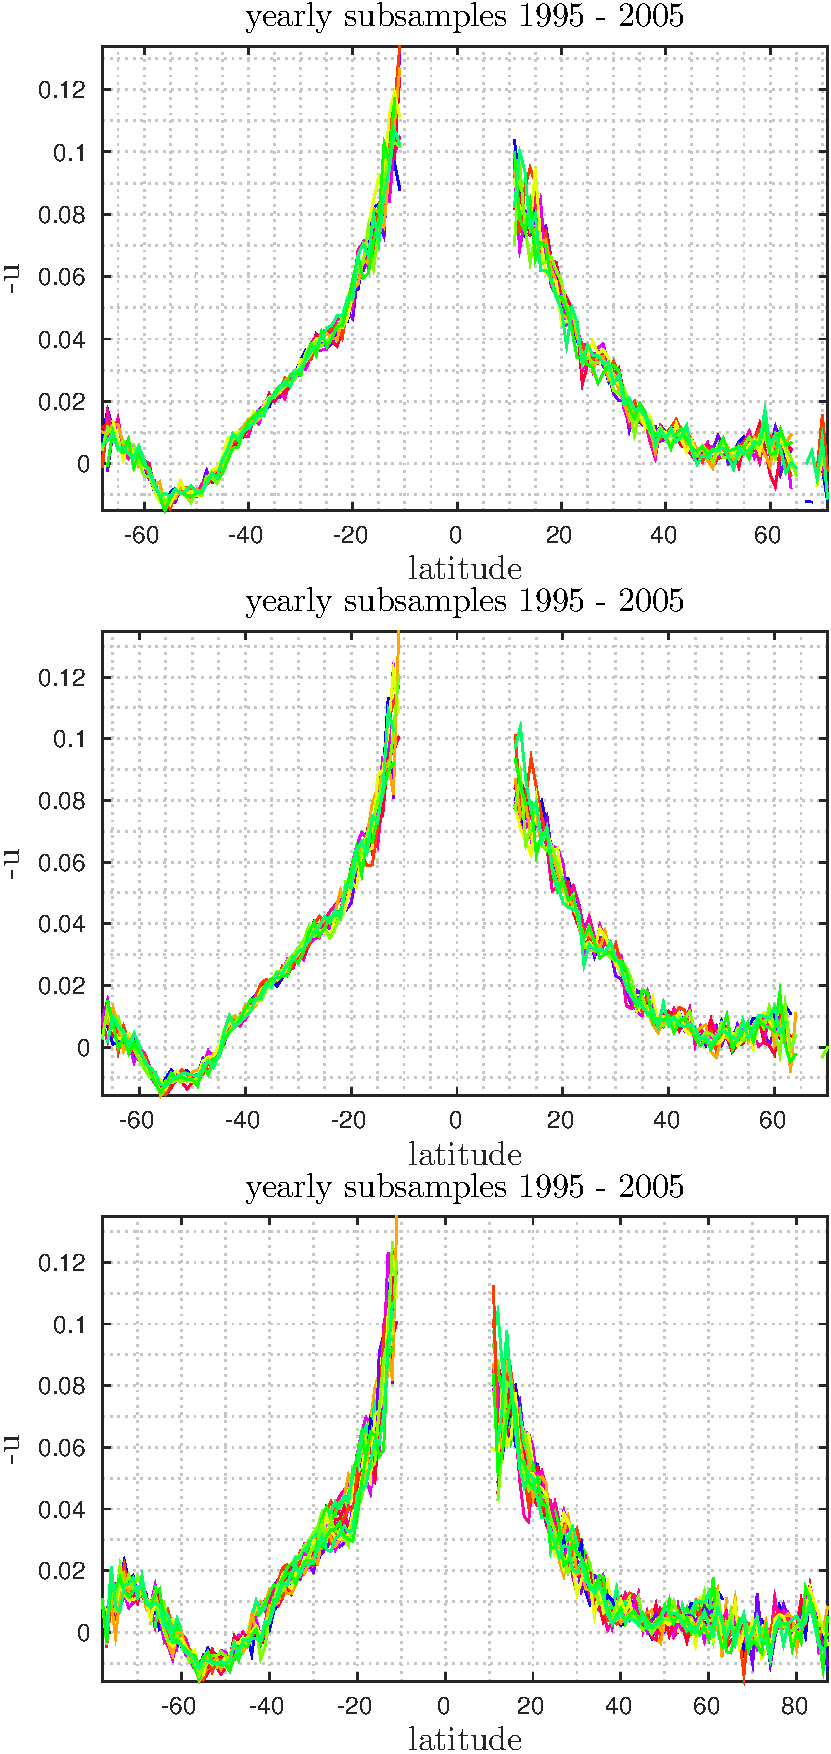
\includegraphics[]{UsubSampledAviIAviIIPop7II}
	\caption{Each line represents zonal means of tracks that ended within one of the eleven years from 1995 to 2005. Top: \aviI. Middle: \aviII. Bottom:  \popSevenII.}
\end{marginfigure}
 %%%%%%%%%%%%%%%%%%%%%%%%%%%%%%%%%%%%%%%%%%%%%%%%%%%%%%%%%%%%%%%%%%%%%%%%%%%%%%%%%

\newthought{The } \popSevenII results yield generally smaller magnitudes of $u$.
The apparent drop in magnitude at $\sim\deg{12}$N is most likely due to erroneous inter-time-step eddy-associations (\cref{fig:ScheltsAll}). In that region, the combination of extreme sparsity of results, large time-step, large $\scale$, low amplitude and high (theoretical) drift speed make robust determinations of $u$ practically impossible.
Yet the tendency for lower magnitudes in $u$, albeit less stark, is also true for higher latitudes.
The zonal drift speeds are calculated via gradients of \textit{poly-fits} to the \CoV-locations on the surface of a spherical earth. This method was tested thoroughly and its robustness is further validated by the fact that the weaker $u$ remains approximately the same after down-sampling for the \pToaII run. Yearly sub-samples of the zonal-mean profiles \footnote{see \cref{fig:UsubSampledAviIAviIIPop7II}.} further prove the consistency of the drift-speeds over time for both data.

% %%%%%%%%%%%%%%%%%%%%%%%%%%%%%%%%%%%%%%%%%%%%%%%%%%%%%%%%%%%%%%%%%%%%%%%%%%%%%%%%%
\newthought{From } \eqref{eq:cush1} we know that at first approximation (planetary lift)
\begin{align}
u
&\sim
\beta \left( 	\frac{NH}{f}  \right)^{2}
\end{align}
Since $\beta, H$ and $f$ should have been set realistically in \POP, it appears that the, evidently unrealistic, drift speeds in the model results stem from an unrealistic or poorly resolved (only 42 vertical layers in \POP) density stratification $\dpr{\rho}{z}$.

\begin{marginfigure}
	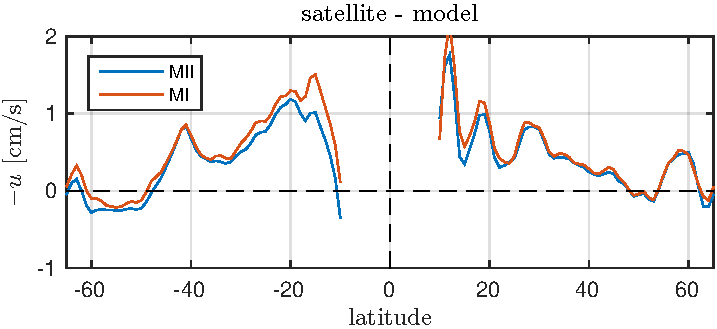
\includegraphics[]{velSatMinusMod}
	\caption{\scriptsize{\aviI/\aviII minus \popSevenII of zonal drift speed means.}}
	\label{fig:velSatMinusMod}
\end{marginfigure}
\newthought{Strong } zonal skewness with opposite sign of $u$ in all analyses (see \cref{fig:SkewAviI}) suggests the existence of many values much smaller in magnitude than the median that smear the distribution of drift speeds towards an unrealistically low mean. This effect appears to be relevant in \eg the Southern Ocean, where the east-ward advection of eddies by the ACC results in a broad spectrum of drift speeds.
The strong gradients in mean current also effect an abundance of eddy~-merging and -splitting situations over relatively short periods of time. It is therefor difficult for the algorithm to keep track of sufficiently long-lived, coherent vortices. Especially so for large time-steps and a high age-threshold. Yet, if the minimum time-step is limited, as in the case of satellite data, a high age-threshold is necessary since short tracks with few data points in time are more likely to stem from erroneously matched contours that do not represent the actual track of a single vortex but instead represent other mesoscale noise that happened to feature sufficiently similar blobs popping in and out of existence at sufficient proximity to one another.


% %%%%%%%%%%%%%%%%%%%%%%%%%%%%%%%%%%%%%%%%%%%%%%%%%%%%%%%%%%%%%%%%%%%%%%%%%%%%%%%%%
\begin{marginfigure}
		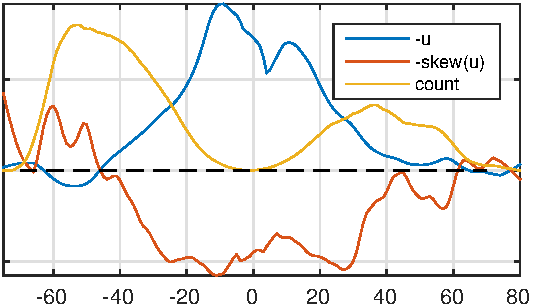
\includegraphics[]{Skew-aviI}
		\caption{\scriptsize{Skewness (red) of $-u$ for \aviI. The spectrum leans towards high westward values in low latitudes. In the ACC the distribution reverses, indicating the existence of sporadic (in time or space (x-dir.)) events of strong eastward advection by the mean flow. (Note: Everything normalized to fit all in one frame.)}}
		\label{fig:SkewAviI}
\end{marginfigure}
% %%%%%%%%%%%%%%%%%%%%%%%%%%%%%%%%%%%%%%%%%%%%%%%%%%%%%%%%%%%%%%%%%%%%%%%%%%%%%%%%%

\newthought{A}~general problem with the depiction of drift-speeds as zonal means is that $u$, besides latitude, is also strongly dependent on longitude. \Cref{fig:MapVisitsBoth-aviII,fig:MapVisitsBoth-pop7II} show strong regional heterogeneity of $u$ presumably influenced by $\f/H$-contours, density stratification and mean flow \citet{Petersen2013,olbers2012ocean}. Note, for example, how the area at $\ang{15}$S west of Australia shows regional drift speeds of $>-\SI{15}{\cm/\s}$ whilst the zonal mean of $u$ amounts to only $\approx -\SI{6}{\cm/s}$. It appears that generally areas of strong eddy-activity yield larger values for $u$ than do areas of weaker mesoscale dynamics (see also \cref{fig:SkewAviI,fig:scat-UampAge-flat-pop7II,fig:TrackPeakampto_ellipseAntiCycsCrpd}).     


\section{\mii~- 2 day time-step - \pop}

So far, all analyses used a $\SI{7}{\day}$-time-step.
As already mentioned in \cref{sec:satvsmod}, from the results we know that eddies translate at speeds on the order $\order{0}\si{\cm\per\s}$~to~$\order{1}\si{\cm\per\s}$ or up to $\SI{100}{\km}/\SI{7}{\day}$ and apparently even more in low latitudes.
This means that one eddy's location might well change as much as its own scale and more over one time-step. Considering how tightly packed eddies often are in areas of high activity, \ie directly adjacent to one another akin to an \textit{egg's box} (see \eg \cref{fig:allEddies-aviIaviIIpop7II}), raises the issue whether the weekly resolution in time is sufficient to successfully track individual eddies and thus deliver realistic translative-speed statistics.
In order to investigate the influence of a shorter time-step the \popSevenII-run was repeated, only this time with a $\SI{2}{\day}$ time-step.
\begin{marginfigure}
	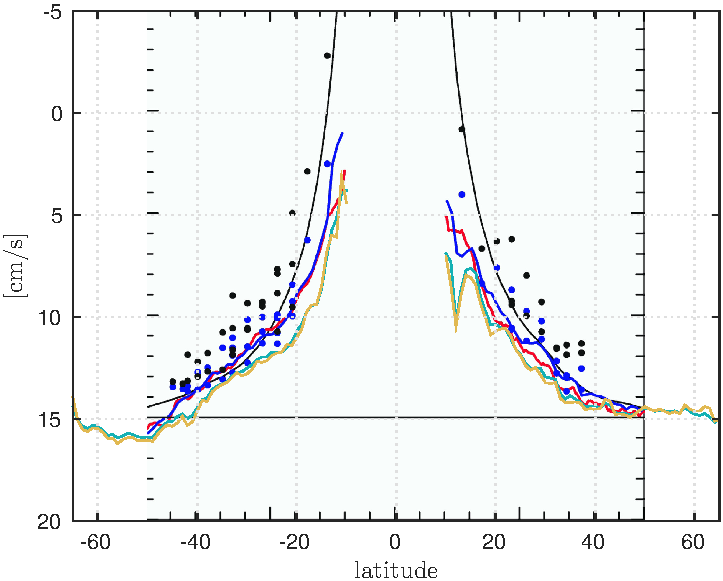
\includegraphics[]{pop2Andpop7velZonMean}
	\caption{Same plot as the \popSevenII~one from \cref{fig:ScheltsAll} with the result from \popTwoII appended in brown. \TODO{refresh}}
	\label{fig:pop2Andpop7velZonMean}
\end{marginfigure}
The effect is only small in the zonal mean (see \cref{fig:pop2Andpop7velZonMean}). But regionally some noteworthy differences to the weekly analysis emerge (see \cref{fig:velZonDiffPopMap}):
\begin{itemize}
\setlength\itemsep{0cm}
	\item 
 Westward drifts are now faster in low latitudes, suggesting that the 7-day time-step is indeed too large to correctly associate all of the large, fast tropical eddies.
 \item
 Areas of strong drift-speed gradients as along the western boundary currents and the ACC show slight general disagreement between the two analyses, suggesting that the analysis benefits from more available time-frames. 
\end{itemize}
\begin{marginfigure}
	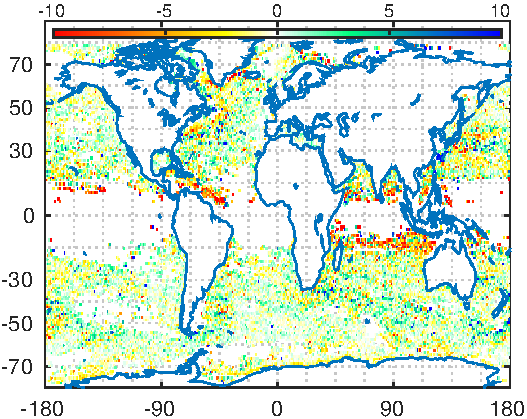
\includegraphics[]{velZonDiffPopMap}
	\caption{Zonal drift speed of \popTwoII minus \popSevenII $\Unit{\si{\cm\per\s}}$. \TODO{update}}
	\label{fig:velZonDiffPopMap}
\end{marginfigure}

\TODO{figure: net U zon mean}

\section{Net Drift Speeds}
\label{sec:netU}
The reversal in drift direction within all sufficiently strong eastward currents (\eg ACC) shows that the, naturally westward-propagating eddies get advected by mean flows, analogous to eastward-moving pressure systems spawned off of the atmospheric jet-stream. Since 3-dimensional current-vectors are available for the model-data, it should be possible to subtract this \textit{Doppler-shift}, in order to extract maps of theoretical drift-speeds without advection by mean-currents. For this to be successful, information about the vertical extent of eddies \ie their \textit{thickness} is indispensable, since horizontal current speeds usually have a significant vertical dependence. The vertical structure of eddies is beyond the scope of this work \footnote{For a discussion of preliminary experiments regarding the vertical structure see \cref{sec:futureTopics}.}. Therefor it was decided to simply average the horizontal background current (time-mean over 2 years) vertically from surface to some depth $z_{bc}$. From the thickness maps of \citet{Petersen2013}, it appears that there are regions with eddy thickness' of $z_{cb}\approx \SI{1000}{\m}$ and regions with $z_{cb} \approx \SI{2000}{\m}$.
Subtracting the constructed background current mean at $z_{cb}$ set to $\SI{2000}{\m}$ from the eddy drift speeds has first and foremost the effect that the net eastweard translation of eddies throughout the ACC disappears.  
This suggests that the tall ACC eddies are indeed simply advected by the deep-reaching background current. The mechanism by which the eddies propagate west (see \cref{box:speed_planlift}) applies relative to the medium it is surrounded by. Both, the planetary-lift- and the $\beta$-internal-effect are independent of the translation vector of the eddy itself.  


\begin{figure}
	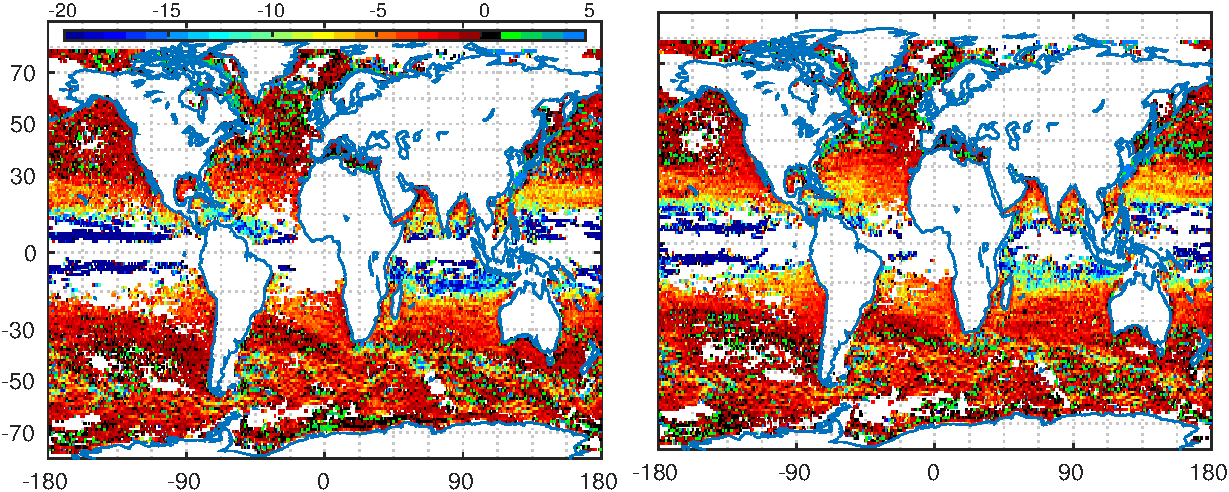
\includegraphics[]{velZonNet1to1000}
	\caption{Zonal drift speed of \popTwoII minus vertical mean from $1\si{\m}$ to $1000\si{\m}$  of mean background current   $\Unit{\si{\cm\per\s}}$. \TODO{update}}
	\label{fig:velZonNet1to1000}
\end{figure}

\begin{figure}
	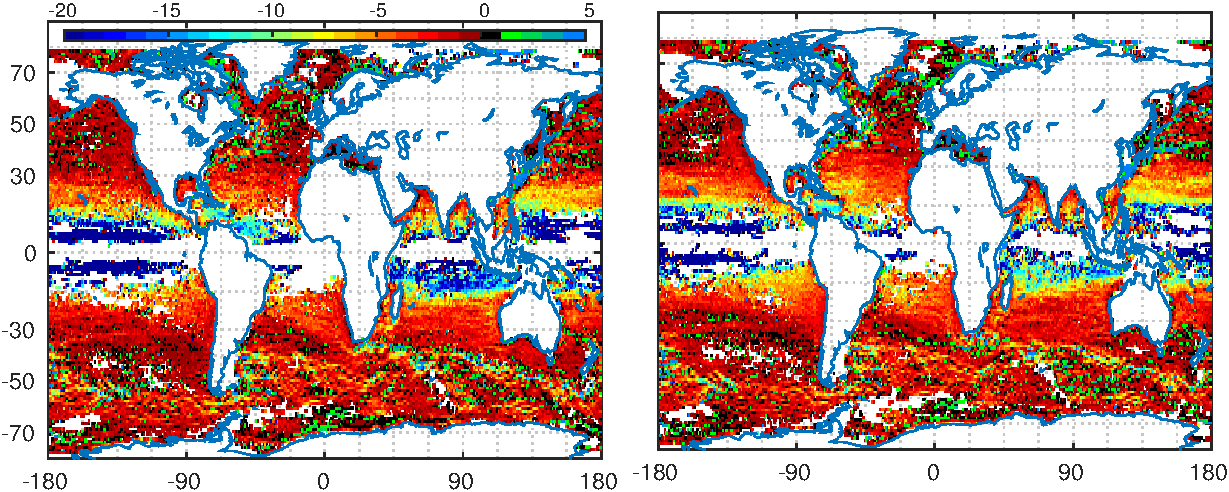
\includegraphics[]{velZonNet1to2000}
	\caption{Zonal drift speed of \popTwoII minus vertical mean from $1\si{\m}$ to $2000\si{\m}$  of mean background current   $\Unit{\si{\cm\per\s}}$. \TODO{update}}
	\label{fig:velZonNet1to2000}
\end{figure}
